\documentclass[a4paper]{article}
\usepackage[utf8]{inputenc}
\usepackage[warn]{mathtext}
\usepackage[russian]{babel}

\usepackage{natbib}

\usepackage{caption}
\usepackage{graphicx}
\graphicspath{}
\DeclareGraphicsExtensions{.pdf,.png,.jpg}
\DeclareSymbolFont{T2Aletters}{T2A}{cmr}{m}{it}
\usepackage{subcaption}

\usepackage{pgfplots}
\pgfplotsset{compat=1.9}

\usepackage{csvsimple}
\usepackage{wrapfig}

\usepackage{svg}
\usepackage{amsmath}
\usepackage{subfiles}

\begin{document}
\begin{minipage}{0.8\textwidth}
\begin{center}
    \large{Санкт-Петербургский национальный исследовательский университет информационных технологий, механики и оптики
\\УЧЕБНЫЙ ЦЕНТР ОБЩЕЙ ФИЗИКИ ФТФ}
\medbreak
\end{center}
\end{minipage}
\hfill
\begin{minipage}{0.3\textwidth}

\includegraphics[scale=0.4]{itmo.jpg}
\end{minipage}

\noindent\rule{\textwidth}{1pt}
\medbreak
\begin{minipage}{0.5\textwidth}
Группа $\textit{P3112}$						
\\Студент $\textit{Сенина Мария Михайловна}$			
\\Преподаватель $\textit{Сорокина Е К}$
\end{minipage}
\hfill
\begin{minipage}{0.4\textwidth}
К работе допущен
\\Работа выполнена
\end{minipage}

\bigbreak

\begin{center}
        \Large{\textbf{Рабочий протокол и отчёт по лабораторной работе № 1.07V}}
   \LARGE{\textbf{\\Маятник Максвелла}}
\end{center}

\section{Цель работы}
Изучение динамики плоского движения твердого тела на примере маятника Максвелла.

\section{Задачи, решаемые при выполнении работы}
\begin{enumerate}
    \item Проверка выполнения закона сохранения энергии маятника с
учетом потерь на отражение и трение.
    \item Определение центрального осевого момента инерции маятника
Максвелла.
\end{enumerate}

\section{Объект исслевдования}
Маятник Максвелла.

\section{Метод экспериментального исследования}
Маятник Максвелла - это массивный диск радиуса $R$ с тонким осевым валом радиусом $r$, который подвешен на двух нитях. Такой маятник совершает плоские колебания вверх и вниз.

\begin{wrapfigure}[10]{r}{0.4\linewidth} 
% \vspace{-5ex}
% 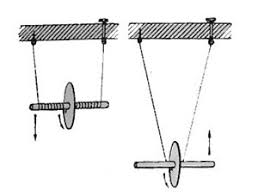
\includegraphics[width=\linewidth]{mayatnik.jpg}
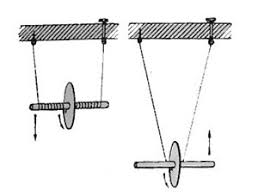
\includegraphics[scale=0.5]{mayatnik.jpg}
\caption{Маятник Максвелла}
\end{wrapfigure}
\medbreak
Момент инерции маятника Максвелла можно найти двумя разными способами - через энегретический и через динамический подходы. 

\medbreak
$\textbf{Динамический подход}$ позволяет рассмотреть движение маятника, как вращательное движение в СО маятника и как поступательное движение в лабораторной системе отсчёта. Тогда второй закон Ньютона для системы можно записать так:
\begin{equation}
    \left\{ 
        \begin{array}{l}
           ma = mg - 2T\\
           I_c \varepsilon = 2Tr\\
        \end{array}
        \right.
    \label{2lawNewton}
\end{equation}
Т.к. нить можно считать нерастяжимой скорость движения центра масс равна скорости вращения диска.
\begin{equation}
    V_{цм} = \omega r
    \label{v=rw}
\end{equation}
Из формул ~\ref{2lawNewton} и ~\ref{v=rw} можно вывести: \[I_c = m r^2(\frac{g}{a}-1)\]

 Аналогичный разультат мы получим пользуясь $\textbf{энергетичкским подходом}$. В для маятника в нижней точке будет выполняться:
 \begin{equation}
     W_{вр} + W_{пост} + \Delta U = 0 \Rightarrow mgh = \frac{mv^2}{2} + \frac{I_c \omega}{2}
    \label{energy}
 \end{equation}
 Зная, что маятник опускается с постоянным ускорением можно понять, что за время $t$ центр масс опустится на $h = \frac{at^2}{2}$, т.к. $v = \omega r$, a $v = at $, $h= \frac{vt}{2} = \frac{\omega r t}{2}$. Подставив это в ~\ref{energy} мы получим ту же формулу для момента инерции маятника  \[ I_c = mr^2 (\frac{gt^2}{2h}-1) = m r^2(\frac{g}{a}-1) \].
 
\section{Рабочие формулы}
\begin{itemize}
    \item Среднее значение 
    \begin{equation}
                \frac{\sum_{i=1}^n x_i}{n}
                \label{average}
            \end{equation}
    \item Момент инерции маятника 
    \begin{equation}
        I_c = mr^2(\frac{gt^2}{2h}-1) = m r^2(\frac{g}{a}-1)
        \label{Ic}
    \end{equation}
    \item Погрешность момента инерции маятника 
    \begin{equation}
        \Delta I_c = S_{\aplha N}\sqrt{(m r^2\Delta \aplha)^2 + ((\aplha - 1)r^2\Delta m)^2 + (2(\aplha-1)m r\Delta r)^2}
        \label{IcPogr}
    \end{equation}
    \item Теоритический момент инерции маятника
    \begin{equation}
        I_{теор} = m R^2
        \label{Ict}
    \end{equation}
    \item  $\alpha$ коэффицент пропорциональности между $I_c$ и $\Delta h$
    \begin{equation}
    \left\{
        \begin{array}{l}
            \frac{gt^2}{2} = \alpha \Delta h\\
            \Delta \alpha = 2\sigma_\aplha\\
            \delta \aplha = \frac{\Delta \alpha}{\aplha}\\
        \end{array}
        \right.
        \label{alpha}
    \end{equation}
    \item Коэфициент уравнения прямой $Y = aX$ через МНК 
        \begin{equation}
            a = \frac{\sum_{i=1}^n x_i\cdot y_i}{\sum_{i=1}^n x^2_i}
            \label{lineMNK}
        \end{equation}
    \item СКО коэффицента $a$ уровнения прямой
    \begin{equation}
           \sigma_a = \sqrt{\frac{\sum_{i=1}^n (y_i - a\cdot x_i)^2}{(N-1)\sum_{i=1}^n x^2_i}}
        \label{MNKpogr}
    \end{equation}
    \item Мгновенная скорость 
    \begin{equation}
        v_i = \frac{2r}{t_i}
        \label{v}
    \end{equation}
    \item Кинетическая энегрия маятника (вращательного и поступательного движения)
    \begin{equation}
        E_к =\frac{m v^2_i}{2}(\frac{I_c}{m r^2} + 1)
        \label{Ek}
    \end{equation}
    \item Потенциальная энергия маятника, если считать за 0 низ его траектории
    \begin{equation}
        E_{пот}=m g h
        \label{Ep}
    \end{equation}
    \item Полная энергия маятника
    \begin{equation}
        E_{полн} = E_{пот} + E_{кин}
        \label{Efull}
    \end{equation}
    \item Погрешность измерений через коэффицент Стьюденса, где $t_{a_{дов, N}}$ - коэффицент Стьюдентса для доверительной вероятности $a_{дов}$ и количества измерений $N$ 
    \begin{equation}
        \Delta x = t_{a_{дов, N}}\sqrt{\frac{\sum\limits_{i=1}^N (x - \bar{x})^2}{N (N-1)}}
        \label{studentskof}
    \end{equation}
\end{itemize}

\section{Измерительные приборы}
$\textbf{Погрешности измерительных приборов}$

\begin{tabular}{ l | l | l | l }\hline
№ & Наименование & Используемый диапазон & Погрешность прибора \\ \hline
1 &	Секундомер & 0.02с - 6.9с & 	0.0001 с \\   \hline
\end{tabular}

\section{Схема установки}

\begin{figure}[h!]
   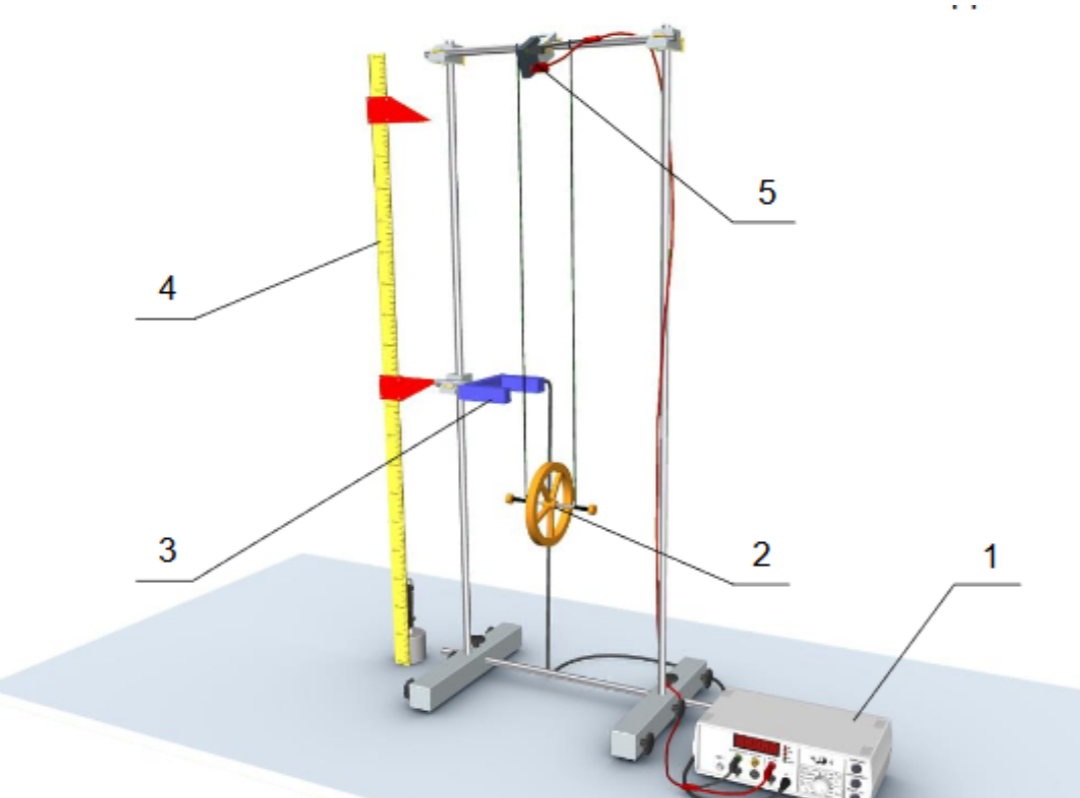
\includegraphics[scale=0.3]{stend.png}
    \caption{Стенд:\\ 1 - цифровой счётчик, 2 - колесо, 3 - рамка с фотоэлементами, 4 - Вертикальная линейка, 5 - Пусковой механизм}
    \label{stend}
\end{figure}

$\textbf{Параметры стенда}$\\
\begin{tabular}{| l | l | l | l | }\hline
№ & Наименование & Значение  & Погрешность\\ \hline
1 & Масса колеса $m$ & 0.47 кг & 0.001 кг \\
2 & Радиус оси колеса $r$ & $2.5 \cdot 10^{-3}$ м & $0.1 \cdot 10^{-3}$ м\\
3 & Радиус маховика $R$ & $0.65$ мм & \\ \hline
\end{tabular}
\newpage
\section{Результаты прямых измерений}
Таблица 1

\begin{tabular}{| l | l | l | l | l | l | l | l |}\hline
$h_0 = 0.1 м$ & $0.2 м$ & $0.3, м$ & $0.4, м$ & $0.5, м$ & $0.6, м$ & $0.7, м$ & $0.8, м$ \\ \hline
$t_1, с$ & 0.200 & 0.300 & 0.400 & 0.500 & 0.600 & 0.700 & 0.800 \\ \hline
$t_2, с$ & 2.614 & 3.713 & 4.563 & 5.265 & 5.896 & 6.463 & 6.978 \\ \hline
$t_3, с$ & 2.615 & 3.720 & 4.561 & 5.270 & 5.894 & 6.460 & 6.984 \\ \hline
$t_4, с$ & 2.614 & 3.720 & 4.562 & 5.270 & 5.898 & 6.463 & 6.972 \\ \hline
$t_5, с$ & 2.613 & 3.715 & 4.557 & 5.264 & 5.893 & 6.454 & 6.982 \\ \hline
$t_6, с$ & 2.614 & 3.719 & 4.561 & 5.265 & 5.896 & 6.456 & 6.973 \\ \hline
\end{tabular}
\medbreak

Таблица 4

\begin{tabular}{| l | l | l | l | l | l | l | l |}\hline
$h_0 = 0.1 м$ & $0.2 м$ & $0.3, м$ & $0.4, м$ & $0.5, м$ & $0.6, м$ & $0.7, м$ & $0.8, м$ \\ \hline
$\Delta h$ & 0.2 & 0.300 & 0.400 & 0.500 & 0.600 & 0.700 & 0.800
$t_1$ & 0.053 & 0.037 & 0.031 & 0.027 & 0.024 & 0.022 & 0.020
$t_2$ & 0.081 & 0.044 & 0.034 & 0.028 & 0.025 & 0.023 & 0.021
$t_3$ & 0.081 & 0.044 & 0.034 & 0.029 & 0.025 & 0.023 & 0.021
\end{tabular}

Измерения проведены в 18:39 4 декабря 2020 года.

\section{Расчёт результатов косвенных измерений}
$\textbf{Часть 1}$

Из данных таблицы 1 посчитаем расстояние $\Delta h = h_0 - h_i$, которое прошёл маятник, от начала движения до рамки с фотоэлементом и среднее время, за которое он это сделал. Зная среднее время движения маятника посчитаем $\frac{gt^2_{ср}}{2}$.

Таблица 2

\begin{tabular}{| l | l | l | l | l | l | l | l |}\hline
$h_0 = 0.1 м$ & $0.2 м$ & $0.3, м$ & $0.4, м$ & $0.5, м$ & $0.6, м$ & $0.7, м$ & $0.8, м$ \\ \hline
$\Delta h, м$ & 0.1 & 0.2 & 0.3 & 0.4 & 0.5 & 0.6 & 0.7 \\ \hline
$t_{ср}, c$ & 2.61 & 3.72 & 4.56 & 5.27 & 5.90 & 6.46 & 6.98 \\ \hline
$\frac{gt^2}{2}$ & 33.55 & 67.85 & 102.13 & 136.19 & 170.66 & 204.85 & 239.05 \\ \hline
\end{tabular}

По формуле $ \frac{gt^2}{2} = \alpha \Delta h$ зависимость $\frac{gt^2_{ср}}{2} (\Delta h)$ - линейна. Тогда построим её график см рис ~\ref{plot1}. Здесь $\alpha$ - коэффицент пропорциональности между $\frac{gt^2_{ср}}{2}$ и $\Delta h$, значит мы можем его вычеслить с помощью метода наименьших квадратов (формулы $ a = \frac{\sum_{i=1}^n x_i\cdot y_i}{\sum_{i=1}^n x^2_i}$ и $\Delta \alpha = \sigma_a * S_t = \sqrt{\frac{\sum_{i=1}^n (y_i - a\cdot x_i)^2}{(N-1)\sum_{i=1}^n x^2_i}}$. 

\[\alpha =  \frac{477.61 \ м^2}{1.40 \ м^2} = 341.2\]
\[\Delta \alpha = \sigma_a S_t = 2 \cdot \sqrt{\frac{0.68 \ м^2}{5 \cdot 1.40 \ м^2 }} = 0.7\]
Значит относительная погрешность $\delta \alpha= \frac{\Delta \alpha}{\aplha} = 0.002 = 0.2\%$

Далее зная $\aplha$ по формулам $I_c = mr^2(\alpha - 1)$ и $\Delta I_c = S_{\aplha N}$ \\ $\sqrt{(m r^2\Delta \aplha)^2 + ((\aplha - 1)r^2\Delta m)^2 + (2(\aplha-1)m r\Delta r)^2}$ мы можем вычислить момент инерции маятника.
\[ I_c = mr^2(\alpha - 1) = 0.47 \ кг \cdot (0.003 \ м)^2 \cdot 341.2 = 1.0 \cdot 10^{-3} кг\cdotм^2\]
\[\Delta I_c = 

\\ 2.77 \sqrt{(0.47 \ кг \cdot (3 \ мм)^2 0.7)^2 + ((341.2 - 1)(3 \ мм)^2 1 \ г)^2 + (2(341.2-1)0.47 \ кг \cdot 30 \cdot 10^{-4} \ м^2)^2} = 0.2 \cdot 10^{-3} кг\cdotм^2 \]


\[ I_c = (1.0 \pm 0.2) \cdot 10^{-3} кг\cdotм^2\]

Теоритически момент инерции должен ровняться $I_{теор} = m R^2 = 2.0 \cdot 10^{-3} кг\cdotм^2$ (по формуле ~\ref{Ict}). 

$\textbf{Часть 2}$

Используя данные из таблицы 3 вычислим мгновенную скорость маятника в каждый из моментов замеров по формуле $v_i = \frac{2r}{t_i}$ (см. таблицу 4). Зная мгновенную скорость вычислим кинетическую энергию маятника в моменты замеров $E_к =\frac{m v^2_i}{2}(\frac{I_c}{m r^2} + 1)$, а зная высоту, на которой зекреплена рамка с фотоэлементом можно вычислить потенциальную энергию $ E_{пот}=m g h$ и полную энергию маятника в этих точках $E_{полн} = E_{пот} + E_{кин}$.

Таблица 4

\begin{tabular}{| l | l | l | l | l | l | l | l |}\hline
$h_0 = 0.1 м$ & $0.2 м$ & $0.3, м$ & $0.4, м$ & $0.5, м$ & $0.6, м$ & $0.7, м$ & $0.8, м$ \\ \hline
$\Delta h$ & 0.1 & 0.2 & 0.3 & 0.4 & 0.5 & 0.6 & 0.7 \\ \hline
$v_1$ & 0.053 & 0.075 & 0.092 & 0.106 & 0.119 & 0.130 & 0.140 \\ \hline
$v_2$ & 0.035 & 0.063 & 0.083 & 0.099 & 0.112 & 0.124 & 0.135 \\ \hline
$v_3$ & 0.035 & 0.063 & 0.083 & 0.098 & 0.112 & 0.123 & 0.134 \\ \hline
$E_k1$ & 0.224 & 0.452 & 0.671 & 0.895 & 1.129 & 1.347 & 1.571 \\ \hline
$E_k2$ & 0.097 & 0.323 & 0.547 & 0.779 & 1.006 & 1.231 & 1.467 \\ \hline
$E_k3$ & 0.096 & 0.320 & 0.550 & 0.763 & 1.006 & 1.220 & 1.439 \\ \hline
$E_пот$ & 3.692 & 3.231 & 2.769 & 2.308 & 1.846 & 1.385 & 0.923 \\ \hline
$E_полн1$ & 3.916 & 3.683 & 3.440 & 3.203 & 2.975 & 2.732 & 2.494 \\ \hline
$E_полн2$ & 3.789 & 3.554 & 3.316 & 3.087 & 2.852 & 2.615 & 2.390 \\ \hline
$E_полн3$ & 3.788 & 3.551 & 3.319 & 3.071 & 2.852 & 2.604 & 2.362 \\ \hline
\end{tabular}
\medbreak
Построим графики зависимости энергии маятника от высоты (см рис ~\ref{plotEfull}).

\section{Окончательные результаты}
Экспериментальный момент инерции маятника
\[ I_c = (1.0 \pm 0.2) \cdot 10^{-3} кг\cdotм^2\] 
Относительная погрешность момента инерции маятника $\delta I_c = 0.22 = 22\%$
Теоритический момент инерции маятника
\[ I_{теор} = m R^2 = 0.2 \cdot 10^{-3} кг\cdotм^2 \]
Получается, что теоритическое значение в два раза больше экспериментального.

Графики зависимости кинетической и полной энергии маятника от высоты (см рис ~\ref{plotEfull}).

\section{Выводы}
В ходе эксперимента мы вычислили момент инерции маятника, с точностью 20\%, но при этом с теоритичесим значением результат расходится в два раза. Это скорее всего происходит потому, что в считая $I_{теор}$ мы считаем ось маятника, к которой крепятся нити полой, а она цельная, т.е. формула $I_{теор} = \frac{mR^2}{2}$. Т.е. результат должнен получиться в два раза меньше и полностью совпасть с экспериментом.

Так же целью эксперимента было проверить выполнения закона сохранения энергии маятника с учетом потерь на отражение и трение. Полная энергия маятника не может сохранятся полностью, т.к. в верёвка, на которую подвешен, маятник не является нерастяжимой и невесомой, что будет приводить к небольшим потерям энергии, особенно в нижней точке. Из графика  (рис ~\ref{E_full}) мы можем заметить, что именно так и происходит. Значения полной энергии в точке $t_1$ и точках $t_2$ и $t_3$ различаются примерно на 0.1 Дж, в то время, как различий в значении у точек $t_2$ и $t_3$ почти нет, как раз потому что маятник проходит нижнюю точку между моментами $t_1$ и $t_2$.

Из графика (рис ~\ref{E_full}) видно, что полная энергия с увеличением высоты полностью не сохраняется, т.к. прямая-аппроксимация значений полной энергии не горизонтальная. К таким результатам могла привести неточность в измерении мгновенной скорости, или пренебрежение потерями энергии из-за растяжимости нити.

\section{Графики}
\begin{figure}[h!]
    \centering
    \includesvg[scale=0.4]{plot1.svg}
    \caption{Зависимость $\frac{gt^2}{2}(\Delta h)$}
    \label{plot1}
\end{figure}

\begin{figure}[h!]
    % \centering
    \includesvg[scale=0.6]{Ek.svg}
    \caption{Зависимость $E_{кин}$ от $h$  для трёх первыйх моментов времени, когда маятник проходит мимо фотодатчика\\ 1) Синий - энергия первого момента 2) Красный - энергия второго момента 3) Зелёный энергия второго момента}
    \label{E_kin}
\end{figure}

\begin{figure}[h!]
    % \centering
    \includesvg[scale=0.6]{Epol.svg}
    \caption{Зависимость $E_{полн}$ от $h$ для трёх первыйх моментов времени, когда маятник проходит мимо фотодатчика\\ 1) Пурпурный - энергия первого момента 2) Светлоголубой - энергия второго момента 3) Жёлтый энергия второго момента}
    \label{E_full}
\end{figure}

\begin{figure}[h!]
    % \centering
    \includesvg[scale=0.31]{plot2.svg}
    \caption{Зависимость $E_{кин}$ и $E_{полн}$ от $h$. Общий график}
    \label{plotEfull}
\end{figure}

% \begin{figure}[h!]
%     % \centering
%     \includesvg[scale=0.5]{EkE1.svg}
%     \caption{Зависимость $E_{кин}$ и $E_{полн}$ от $h$, для первого замера времени}
%     \label{E1}
% \end{figure}

% \begin{figure}[h!]
%     % \centering
%     \includesvg[scale=0.5]{EkE2.svg}
%     \caption{Зависимость $E_{кин}$ и $E_{полн}$ от $h$, для второго замера времени}
%     \label{E2}
% \end{figure}

% \begin{figure}[h!]
%     % \centering
%     \includesvg[scale=0.5]{EkE3.svg}
%     \caption{Зависимость $E_{кин}$ и $E_{полн}$ от $h$, для третьего замера времени}
%     \label{E3}
% \end{figure}



\end{document}